\documentclass[border=0pt]{standalone}
\usepackage[T1]{fontenc}
\usepackage{lmodern}
\usepackage{pgfplots}
\usepgfplotslibrary{groupplots}
\pgfplotsset{compat=1.18}
\definecolor{f02sg}{HTML}{0072B2}
\definecolor{f02arpls}{HTML}{D55E00}
\begin{document}
\begin{minipage}{181.86mm}
\centering
{\bfseries\fontsize{10}{12}\selectfont P08-F02 Extra Trees / M06 combined predictions per physical sample / Sensitivity (S)}\par\vspace{6mm}
% semantic SHA-256: 4c3507299219d2ce29fd9a2a58f030be1b778fd9bbceb756756ca16d12f674f7
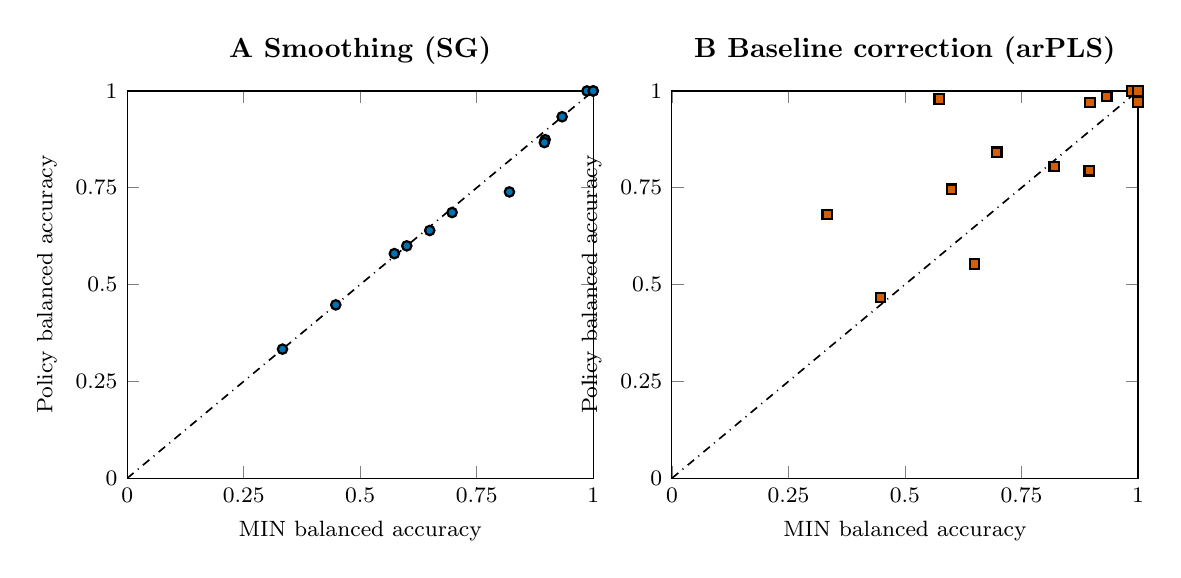
\begin{tikzpicture}
\begin{groupplot}[
  group style={group size=2 by 1, horizontal sep=10mm, vertical sep=6mm},
  width=75mm, height=65mm,
  xmin=0, xmax=1, ymin=0, ymax=1,
  xtick={0,0.25,0.5,0.75,1}, ytick={0,0.25,0.5,0.75,1},
  tick label style={font=\fontsize{8}{9}\selectfont},
  label style={font=\fontsize{8}{9}\selectfont},
  title style={font=\bfseries\fontsize{10}{12}\selectfont},
  xlabel={MIN balanced accuracy}, ylabel={Policy balanced accuracy},
]
\nextgroupplot[title={A  Smoothing (SG)}]
\addplot[black, dash dot, line width=0.6pt, samples=2, domain=0:1, forget plot] {x};
\addplot[only marks, mark=*, mark size=1.7pt, color=f02sg, mark options={draw=black,line width=0.8pt}] coordinates {(0.8202380952380952,0.7392857142857142) (0.6492063492063492,0.6396825396825397) (0.6972222222222222,0.6861111111111111) (0.9866666666666667,1.0) (1.0,1.0) (0.3333333333333333,0.3333333333333333) (0.9333333333333332,0.9333333333333332) (1.0,1.0) (0.44761904761904764,0.44761904761904764) (0.6,0.6) (0.8969696969696971,0.8742424242424243) (0.8952380952380953,0.8666666666666666) (0.5733333333333334,0.58)};
\nextgroupplot[title={B  Baseline correction (arPLS)}]
\addplot[black, dash dot, line width=0.6pt, samples=2, domain=0:1, forget plot] {x};
\addplot[only marks, mark=square*, mark size=1.7pt, color=f02arpls, mark options={draw=black,line width=0.8pt}] coordinates {(0.8202380952380952,0.8044973544973546) (0.6492063492063492,0.5531746031746031) (0.6972222222222222,0.8416666666666666) (0.9866666666666667,1.0) (1.0,1.0) (0.3333333333333333,0.680952380952381) (0.9333333333333332,0.9866666666666667) (1.0,0.9714285714285715) (0.44761904761904764,0.4666666666666667) (0.6,0.7460317460317459) (0.8969696969696971,0.9696969696969697) (0.8952380952380953,0.7936507936507936) (0.5733333333333334,0.9792592592592593)};
\end{groupplot}
\end{tikzpicture}
\par\vspace{4pt}
{\fontsize{8}{10}\selectfont RQ-S01: preprocessing and chemical identification. Source-only selection/calibration; selected CNN identity fixed across policies. SG = impulse replacement, smoothing, minmax; arPLS = impulse replacement, baseline correction, minmax. MIN = minimal minmax. Primary: equal contexts within domain, then equal domains. Pooled-fold sensitivity reconstructs each four-fold prediction set before scoring. M01 individual-spectrum predictions; M06 combined predictions per physical sample. M06 averages model probabilities within sample/instrument then equally across instruments, never input spectra or hard labels. 598 original spectra / 69 physical samples / 10 instruments; 557 spectra in 13 held station/instrument domains, 260 contexts. Per-domain independent support in the CSV/table. D1..D13 are lexicographic station/instrument domains, not samples. Diagonal y=x; the 520 points across all panels are paired domain measurements, not 520 independent observations. Claim limit: cannot establish causal background removal or new-instrument performance; no error bars, no significance stars.}\par
\end{minipage}
\end{document}